%!TEX program = xelatex
\documentclass[a4paper, 12pt, UTF8]{ctexart}
\usepackage[english]{babel}
\usepackage[utf8]{inputenc}
\usepackage{johd}
\usepackage{ctex}
\usepackage{amsmath}
\usepackage{graphicx}
\usepackage{caption}
\usepackage{subcaption} 
\usepackage{amssymb}
\newcommand{\bs}[1]{\boldsymbol{#1}}

\title{空气动力学方程组间断有限元方法}

\date{} %leave blank

\begin{document}

\maketitle


\section{方程简介}
考虑三维Euler方程组, 将其写成双曲守恒律形式:
\begin{equation}
 \begin{cases}
    	\bs {u_{t}}+\nabla \cdot \bs f(\bs u)=0 \\
    	\bs u(x, y, z, 0)=\bs{u_{0}}(x, y, z)
    \end{cases} \quad (x, y, z, t)  \in \Omega \times(0, T)
\end{equation}
其中,$\bs u$为守恒量,$\bs f(u)=\left(f_{1}(u), f_{2}(u), f_{3}(u)\right)$ 为通量,
\begin{equation}
\bs{u}=\begin{bmatrix}
	u_0\\
	u_{1}\\
	u_{2}\\
	u_{3}\\
	u_4
\end{bmatrix}
=\begin{bmatrix}
	\rho\\
	\rho v_{1}\\
	\rho v_{2}\\
	\rho v_{3}\\
	 E
\end{bmatrix}
\quad f_{1}(\bs{u})=\begin{bmatrix}
	\rho v_{1}\\
	\rho v_{1}^{2}+p\\
	\rho v_{2} v_{1}\\
	\rho v_{3} v_{1}\\
	(E+p) v_{1}
\end{bmatrix},
\quad f_{2}(\bs{u})=\begin{bmatrix}
	 \rho v_{2}\\
	 \rho v_{1} v_{2}\\
	 \rho v_{2}^{2}+p\\
	 \rho v_{3} v_{2}\\
	 (E+p) v_{2}
\end{bmatrix},
\quad f_{3}(\bs{u})=\begin{bmatrix}
	 \rho v_{3}\\
	 \rho v_{1} v_{3}\\
	 \rho v_{2} v_{3}\\
	 \rho v_{3}^{2}+p\\ 
	 (E+p) v_{3}
\end{bmatrix}
\end{equation}
其中,$\rho$ 表示密度,$\bs{v} = (v_{1}, v_{2}, v_{3})$ 为速度,E为能量,压力 
\begin{equation}\label{pressure}
p=(\gamma-1)\left(E-\frac{1}{2} \rho\bs{||v||}^{2}\right)=(\gamma-1)\left(u_4-\frac{1}{2u_0} \left(u_1^{2}+u_{2}^{2}+u_{3}^{3}\right)\right)
\end{equation}
绝热指数 $\gamma$在计算中一般取为常数1.4。

下面给出二维Euler方程的一个有光滑解的例子,常用来测试算法的精度。在该例子中, 计算区域$\Omega=[0,2]^3$,给定 
初始条件: 
\begin{equation}
\begin{cases}
	   \rho(x, y, z, 0)=1+0.2 \sin (\pi(x+y+z)) \\
	   v_{1}(x, y, z, 0)=0.4, \quad v_{2}(x, y, z, 0)=0.3  \\
	   v_{3}(x, y, z, 0)=0.3, \quad p(x, y, z, 0)=1 
    \end{cases}
\end{equation}
取周期边界条件,则密度函数有精确解:
$$\rho(x, y, z, t)=1+0.2 \sin (\pi(x+y+z-t)) $$
该算例一般可以计算到$T = 2$。




\section{基函数与外法向量}
设$\mathcal T_h=\{K\}$为区域$\Omega$的一个四面体剖分,在$\mathcal T_h$中的任意一个四面体$K$上,设$\{(x_i,y_i,z_i)\}_{i=0}^3$为四面体的四个顶点的坐标,如图\ref{tetrahedron}所示。

设四面体单元K的体积为V,P为四面体内一点,四面体$PA_{1}A_{2}A_{3}$,$PA_{0}A_{2}A_{3}$,$PA_{0}A_{1}A_{3}$的体积分别为$V_{0}$,$V_{1}$,$V_{2}$,则有
\begin{equation}
\begin{split}
6 V=\left|\begin{array}{cccc}
1 & x_{0} & y_{0} & z_{0} \\
1 & x_{1} & y_{1} & z_{1} \\
1 & x_{2} & y_{2} & z_{2} \\
1 & x_{3} & y_{3} & z_{3}
\end{array}\right| , \quad
6 V_{0}=\left|\begin{array}{cccc}
1 & x & y & z \\
1 & x_{1} & y_{1} & z_{1} \\
1 & x_{2} & y_{2} & z_{2} \\
1 & x_{3} & y_{3} & z_{3}
\end{array}\right| , \\
6 V_{1}=\left|\begin{array}{cccc}
1 & x_{0} & y_{0} & z_{0} \\
1 & x & y & z \\
1 & x_{2} & y_{2} & z_{2} \\
1 & x_{3} & y_{3} & z_{3}
\end{array}\right| ,  \quad
6 V_{2}=\left|\begin{array}{cccc}
1 & x_{0} & y_{0} & z_{0} \\
1 & x_{1} & y_{1} & z_{1} \\
1 & x & y & z \\
1 & x_{3} & y_{3} & z_{3} 
\end{array}\right| .
\end{split}
\end{equation}

令:$\eta_{0} = V_{0}/V$,$\eta_{1} = V_{1}/V$,$\eta_{2} = V_{2}/V$,其中
\begin{equation}
\begin{split}
&\nabla \eta _{0}=\frac{1}{6 V}\left(-\left|\begin{array}{lll}
1 & y_{1} & z_{1} \\
1 & y_{2} & z_{2} \\
1 & y_{3} & z_{3}
\end{array}\right|, \left|\begin{array}{lll}
1 & x_{1} & z_{1} \\
1 & x_{2} & z_{2} \\
1 & x_{3} & z_{3}
\end{array}\right|, -\left|\begin{array}{ccc}
1 & x_{1} & y_{1} \\
1 & x_{2} & y_{2} \\
1 & x_{3} & y_{3}
\end{array}\right|\right) \\[2pt]
&\nabla \eta_{1}=\frac{1}{6 V}\left(\left|\begin{array}{lll}
1 & y_{0} & z_{0} \\
1 & y_{2} & z_{2} \\
1 & y_{3} & z_{3}
\end{array}\right|, -\left|\begin{array}{lll}
1 & x_{0} & z_{0} \\
1 & x_{2} & z_{2} \\
1 & x_{3} & z_{3}
\end{array}\right|, \left|\begin{array}{ccc}
1 & x_{0} & y_{0} \\
1 & x_{2} & y_{2} \\
1 & x_{3} & y_{3}
\end{array}\right|\right) \\[2pt]
&\nabla \eta_{2}=\frac{1}{6 V}\left(-\left|\begin{array}{lll}
1 & y_{0} & z_{0} \\
1 & y_{1} & z_{1} \\
1 & y_{3} & z_{3}
\end{array}\right|, \left|\begin{array}{lll}
1 & x_{0} & z_{0} \\
1 & x_{1} & z_{1} \\
1 & x_{3} & z_{3}
\end{array}\right|, -\left|\begin{array}{ccc}
1 & x_{0} & y_{0} \\
1 & x_{1} & y_{1} \\
1 & x_{3} & y_{3}
\end{array}\right|\right)
\end{split}
\end{equation}

\begin{figure}[!ht]
\centering
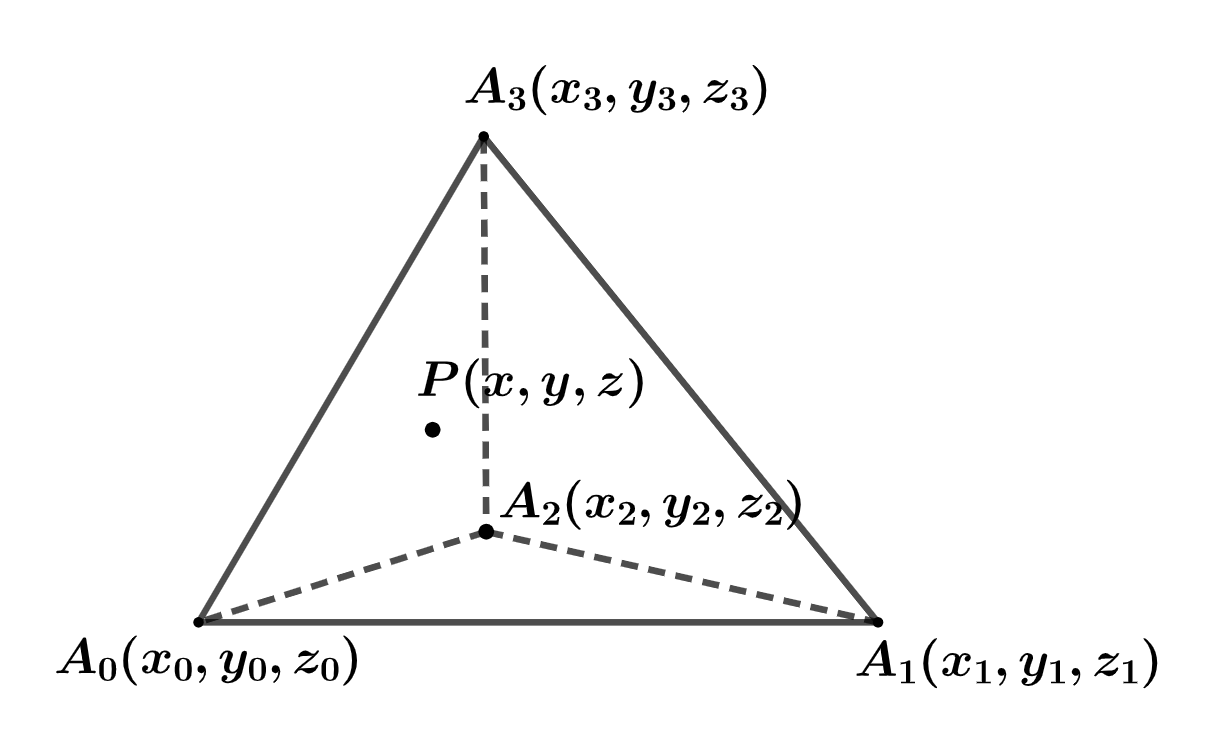
\includegraphics[width=0.52\textwidth]{images/1.png}
\caption{四面体单元}
\label{tetrahedron}
\end{figure}

通过体积坐标变换:
\begin{equation}
\left(\begin{array}{l}
x \\
y \\
z
\end{array}\right)=\eta_{0}\left(\begin{array}{l}
x_{0} \\
y_{0} \\
z_{0}
\end{array}\right)+\eta_{1}\left(\begin{array}{l}
x_{1} \\
y_{1} \\
z_{1}
\end{array}\right)+\eta_{2}\left(\begin{array}{l}
x_{2} \\
y_{2} \\
z_{2}
\end{array}\right)+\left(1-\eta_{0}-\eta_{1}-\eta_{2}\right)\left(\begin{array}{l}
x_{3} \\
y_{3} \\
z_{3}
\end{array}\right)
\end{equation}

可将单元K变换到标准四面体单元:
\begin{equation}
\hat{K}=\left\{\boldsymbol{\eta}=\left(\eta_{0}, \eta_{1}, \eta_{2}\right) \mid \eta_{0}+\eta_{1}+\eta_{2} \leqslant 1, 0 \leqslant \eta_{0}, \eta_{1}, \eta_{2} \leqslant 1\right\}
\end{equation}

在参考单元 $\hat{K}$ 上考虑一次多项式空间,可以得到四个相互正交的基函数如下:
\begin{equation}	
\begin{split}
&\hat{\varphi}_{0} = 1, \quad
\hat{\varphi}_{1} = -\frac{1}{4} + \eta_{0}, \quad
\hat{\varphi}_{2} = -\frac{1}{3} + \frac{1}{3} \eta_{0} + \eta_{1}, \\
&\hat{\varphi}_{3} = -\frac{1}{2} + \frac{1}{2} \eta_{0} + \frac{1}{2} \eta_{1} + \eta_{2}.
\end{split}
\end{equation}

在参考单元上定义 $L^{2}$ 内积 $\left(\hat{\varphi}_{i}, \hat{\varphi}_{j}\right)=\int_{\hat{K}} \hat{\varphi}_{i} \hat{\varphi}_{j} d \bs{\eta}$,经过简单计算有:
\begin{equation}
\begin{split}
\left(\hat{\varphi}_{i}, \hat{\varphi}_{j}\right) &= 0 \quad (i \neq j), \quad 
\left(\hat{\varphi}_{0}, \hat{\varphi}_{0}\right) = \frac{1}{6}, \quad
\left(\hat{\varphi}_{1}, \hat{\varphi}_{1}\right) = \frac{1}{160}, \\
\left(\hat{\varphi}_{2}, \hat{\varphi}_{2}\right) &= \frac{1}{180}, \quad
\left(\hat{\varphi}_{3}, \hat{\varphi}_{3}\right) = \frac{1}{240}.
\end{split}
\end{equation}

利用这些基函数,我们可以在单元K上定义$\bs{u}$的近似
\begin{equation}\label{numericsolution}
\bs u_{h}^K(\boldsymbol{X}, t)=\sum\limits_{j=0}^{3} \bs u_{j}^K(t) \varphi_{j}^K(\boldsymbol{X}) \quad \boldsymbol{X} = (x, y, z) \in K
\end{equation}

其中,$\varphi_{j}^{K}(\boldsymbol{X})=\hat{\varphi}_{j}(\bs{\eta}(\boldsymbol{X}))$,
因为
\begin{equation}\label{othorgnal}
\int_{K}\left(\varphi_{j}^{K}\right)^{2} d\bs{X} = \int_{\hat{K}}\hat{\varphi_{j}}^{2} |J|d\bs{\eta} = |J|\left(\hat{\varphi}_{j}, \hat{\varphi}_{j}\right)
\end{equation}

$|J| = 6|K|$ 为Jacobian矩阵行列式的绝对值,所以$\varphi_{j}^K(\boldsymbol{X})$也是单元K上的正交基函数。

设$\bs n_{0}$, $\bs n_{1}$, $\bs n_{2}$, $\bs n_{3}$ 分别表示为单元$K$四个顶点$A_{0}, A_{1}, A_{2}, A_{3}$所对的面上的单位外法向量,下面以$\bs n_{0}$为例来说明它的计算方法:
\begin{equation}
\begin{split}
&\bs{A_{1} A_{2}} = \left(x_{2}-x_{1}, y_{2}-y_{1}, z_{2}-z_{1}\right) \quad
\bs{A_{1} A_{3}}=\left(x_{3}-x_{1}, y_{3}-y_{1}, z_{3}-z_{1}\right) \\
&\bs{A_{1} A_{2}} \times \bs{A_{1} A_{3}} =\left(\left|\begin{array}{ll}
y_{2}-y_{1} & z_{2}-z_{1} \\
y_{3}-y_{1} & z_{3}-z_{1}
\end{array}\right|,-\left|\begin{array}{ll}
x_{2}-x_{1} & z_{2}-z_{1} \\
x_{3}-x_{1} & z_{3}-z_{1}
\end{array}\right|,\left|\begin{array}{ll}
x_{2}-x_{1} & y_{2}-y_{1} \\
x_{3}-x_{1} & y_{3}-y_{1}
\end{array}\right|\right) \\
&\bs{A_{1} A_{0}} = \left(x_{0}-x_{1}, y_{0}-y_{1}, z_{0}-z_{1}\right) \\[3mm] 
&\bs{n_{0}} = \left\{
\begin{array}{ll}
\frac{\displaystyle \bs{A_{1} A_{2}} \times \bs{A_{1} A_{3}}}{\left| \displaystyle \bs{A_{1} A_{2}} \times \bs{A_{1} A_{3}}\right|} & \left(\bs{A_{1} A_{2}} \times \bs{A_{1} A_{3}}\right) \cdot \bs{A_{1} A_{0}} < 0, \\[5mm] 
-\frac{\displaystyle \bs{A_{1} A_{2}} \times \bs{A_{1} A_{3}}}{\left| \displaystyle \bs{A_{1} A_{2}} \times \bs{A_{1} A_{3}}\right|} & \left(\bs{A_{1} A_{2}} \times \bs{A_{1} A_{3}}\right) \cdot \bs{A_{1} A_{0}} > 0.
\end{array}
\right.
\end{split}
\end{equation}


\newpage

\section{DG格式的空间离散}

为了求得在任意三角形单元$K$上的近似解  
\begin{equation}\label{spacediscritization}
\bs u^K_{h}(\bs{X}, t)=\sum\limits_{j=0}^{3} \bs u^K_{j}(t) \varphi_{j}^K(\bs{X})
\end{equation}
我们要求近似解$\bs u^K_h(\bs{X}, t)$在$K$上满足方程
\begin{equation}
\int_K\frac{d}{d t} \bs u_{h}^K(\bs{X}, t)\varphi_j^Kd\bs{X}=\int_K\bs f(\bs u_{h}^K(\bs{X}, t))\cdot\nabla\varphi_j^Kd{\bs{X}}-\int_{\partial K}\hat{\bs f}(\bs{X}, t)\varphi_j^Kds
\end{equation}
其中$j=0, 1, 2, 3$, $\hat{\bs f}(\bs{X}, t)$为人为定义的数值通量,将在后面给出具体的定义。将表达式\eqref{numericsolution}代入上式,并应用性质\eqref{othorgnal}得,系数$\bs u_{j}^K(t)$ 满足常微分方程组:
\begin{equation}\label{semidiscrete}
 \frac{d}{d t} \bs u_{j}^K(t)=\frac{1}{a_{j}}\left[\int_{K} {\bs f}\left(\bs u_{h}^K(\bs{X}, t)\right) \cdot \nabla \varphi_{j}^Kd\bs{X}\right. \left.-\int_{\partial K}\hat{\bs f}\left(\bs{X}	, t\right) \varphi_{j}^K d s\right] 
\end{equation}
其中,$a_{j}=\int_{K}\left(\varphi_{j}^{K}(\bs{X})\right)^{2} d\bs{X} = \int_{\hat{K}}\hat{\varphi_{j}}^{2}(\bs{\eta}) |J|d\bs{\eta} = |J|\left(\hat{\varphi}_{j}, \hat{\varphi}_{j}\right)$。

方程右端的积分项可以用数值求积公式来进行计算:
\begin{equation}
\begin{split}
\int_{K} \bs f\left(\bs u_{h}^K(\bs{X}, t)\right) \cdot  \nabla \varphi_{j}^K(\bs{X}) &d \bs{X} 
\approx |K| \sum_{m=0}^{3} \frac{1}{4} \bs f\left(\bs u_{h}^K\left(\hat{\bs{X}}_{m}^K,  t\right)\right) \cdot \nabla \varphi_{j}^K\left(\hat{\bs{X}}_{m}^K\right)\\
\end{split}
\end{equation}

其中,$\bs{u}_{h}^{K}\left(\hat{\bs{X}}^{K}_{m}, t\right)=\sum\limits_{j=0}^{3} \bs{u}_{j}^{K}(t) \varphi_{j}^{K}\left(\hat{\bs{X}}^{K}_{m}\right)=\sum\limits_{j=0}^{3} \bs{u}_{j}^{K}(t) \hat{\varphi}_{j}\left(\hat{\bs{\eta}}_{m}\right)$

$\hat{\bs{\eta}}_{m}$ 为标准单元内的求积节点,有$\hat{\bs{\eta}}_{0}=(\alpha, \beta, \beta)$,$\hat{\bs{\eta}}_{1}=(\beta,\alpha,  \beta)$,$\hat{\bs{\eta}}_{2}=(\beta, \beta, \alpha)$,$\hat{\bs{\eta}}_{3}=(\beta, \beta, \beta)$,参数$\alpha=0.58541020$,$\beta=0.13819660$。
\begin{equation}
\nabla \varphi_j^{K}(\hat{\bs{X}}_{m}) =
\left(
\frac{\partial \varphi_j}{\partial x}, 
\frac{\partial \varphi_j}{\partial y}, 
\frac{\partial \varphi_j}{\partial z}
\right) 
= 
\left(
\frac{\partial \hat{\varphi}_j}{\partial \eta_0}, 
\frac{\partial \hat{\varphi}_j}{\partial \eta_1}, 
\frac{\partial \hat{\varphi}_j}{\partial \eta_2}
\right)
\begin{pmatrix}
\frac{\partial \eta_0}{\partial x} & \frac{\partial \eta_0}{\partial y} & \frac{\partial \eta_0}{\partial z} \\
\frac{\partial \eta_1}{\partial x} & \frac{\partial \eta_1}{\partial y} & \frac{\partial \eta_1}{\partial z} \\
\frac{\partial \eta_2}{\partial x} & \frac{\partial \eta_2}{\partial y} & \frac{\partial \eta_2}{\partial z}
\end{pmatrix}
\end{equation}
\begin{equation}
\begin{split}
&\int_{\partial K} \hat{\bs{f}}(\bs{X}, t) \varphi_{j}^K(\bs{X}) d s =\sum_{i=0}^{3} \int_{\partial K_{i}} \hat{\bs{f}}(\bs{X}, t) \varphi_{j}^K(\bs{X}) d s \\
&\approx \sum_{i=0}^{3}\left(\left|\partial K_{i}\right| \sum_{m=0}^{2} \frac{1}{3} \hat{\bs{f}}\left(\bar{\bs{X}}^{\partial K_{i}}_{m}, t\right) \varphi_{j}^K\left(\bar{\bs{X}}_{m}^{\partial K_{i}}\right)\right) =
 \sum_{i=0}^{3}\left(\left|\partial K_{i}\right| \sum_{m=0}^{2} \frac{1}{3} \hat{\bs{f}}\left(\bar{\bs{X}}^{\partial K_{i}}_{m}, t\right) \hat{\varphi}_{j}\left(\bar{\bs{\eta}}_{m}^{\partial K_{i}}\right)\right)
\end{split}
\end{equation}

其中,$\bar{\bs{\eta}}_{m}^{\partial K_{i}}$为标准单元边界 $\partial K_{i}$上的求积节点,$|\partial K_{i}|$表示面积,如图\ref{IntegrationBoundaryPoint}。
\begin{equation}
\begin{split}
\bar{\bs{X}}_{0}^{\partial K_{3}}=\frac{2}{3} \bs{X}_{0}+\frac{1}{6} \bs{X}_{1}+\frac{1}{6} \bs{X}_{2} & \quad \bar{\bs{\eta}}_{0}^{\partial K_{3}}=\left(\frac{2}{3}, \frac{1}{6}, \frac{1}{6}\right) \\
\bar{\bs{X}}_{1}^{\partial K_{3}}=\frac{1}{6} \bs{X}_{0}+\frac{2}{3} \bs{X}_{1}+\frac{1}{6} \bs{X}_{2} & \quad \bar{\bs{\eta}}_{1}^{\partial K_{3}}=\left(\frac{1}{6}, \frac{2}{3}, \frac{1}{6}\right) \\
\bar{\bs{X}}_{2}^{\partial K_{3}}=\frac{1}{6} \bs{X}_{0}+\frac{1}{6} \bs{X}_{1}+\frac{2}{3} \bs{X}_{2} & \quad \bar{\bs{\eta}}_{2}^{\partial K_{3}}=\left(\frac{1}{6}, \frac{1}{6}, \frac{2}{3}\right)
\end{split}
\end{equation} 

类似的,可以得到$\partial K_{2}, \partial K_{1}, \partial K_{0}$上求积节点的体积坐标:
\begin{equation}
\begin{split}
\bar{\bs{\eta}}_{0}^{\partial K_{2}}=\left(\frac{2}{3}, \frac{1}{6}, 0\right) \quad \bar{\bs{\eta}}_{1}^{\partial K_{2}}=\left(\frac{1}{6}, \frac{2}{3}, 0\right) \quad \bar{\bs{\eta}}_{2}^{\partial K_{2}}=\left(\frac{1}{6}, \frac{1}{6}, 0\right) \\
\bar{\bs{\eta}}_{0}^{\partial K_{1}}=\left(\frac{2}{3}, 0, \frac{1}{6}\right) \quad \bar{\bs{\eta}}_{1}^{\partial K_{1}}=\left(\frac{1}{6}, 0, \frac{2}{3}\right) \quad \bar{\bs{\eta}}_{2}^{\partial K_{1}}=\left(\frac{1}{6}, 0, \frac{1}{6}\right) \\
\bar{\bs{\eta}}_{0}^{\partial K_{0}}=\left(0, \frac{2}{3}, \frac{1}{6}\right) \quad \bar{\bs{\eta}}_{1}^{\partial K_{0}}=\left(0, \frac{1}{6}, \frac{2}{3}\right) \quad \bar{\bs{\eta}}_{2}^{\partial K_{0}}=\left(0, \frac{1}{6}, \frac{1}{6}\right)
\end{split}
\end{equation}


\begin{figure}[!ht]
\centering
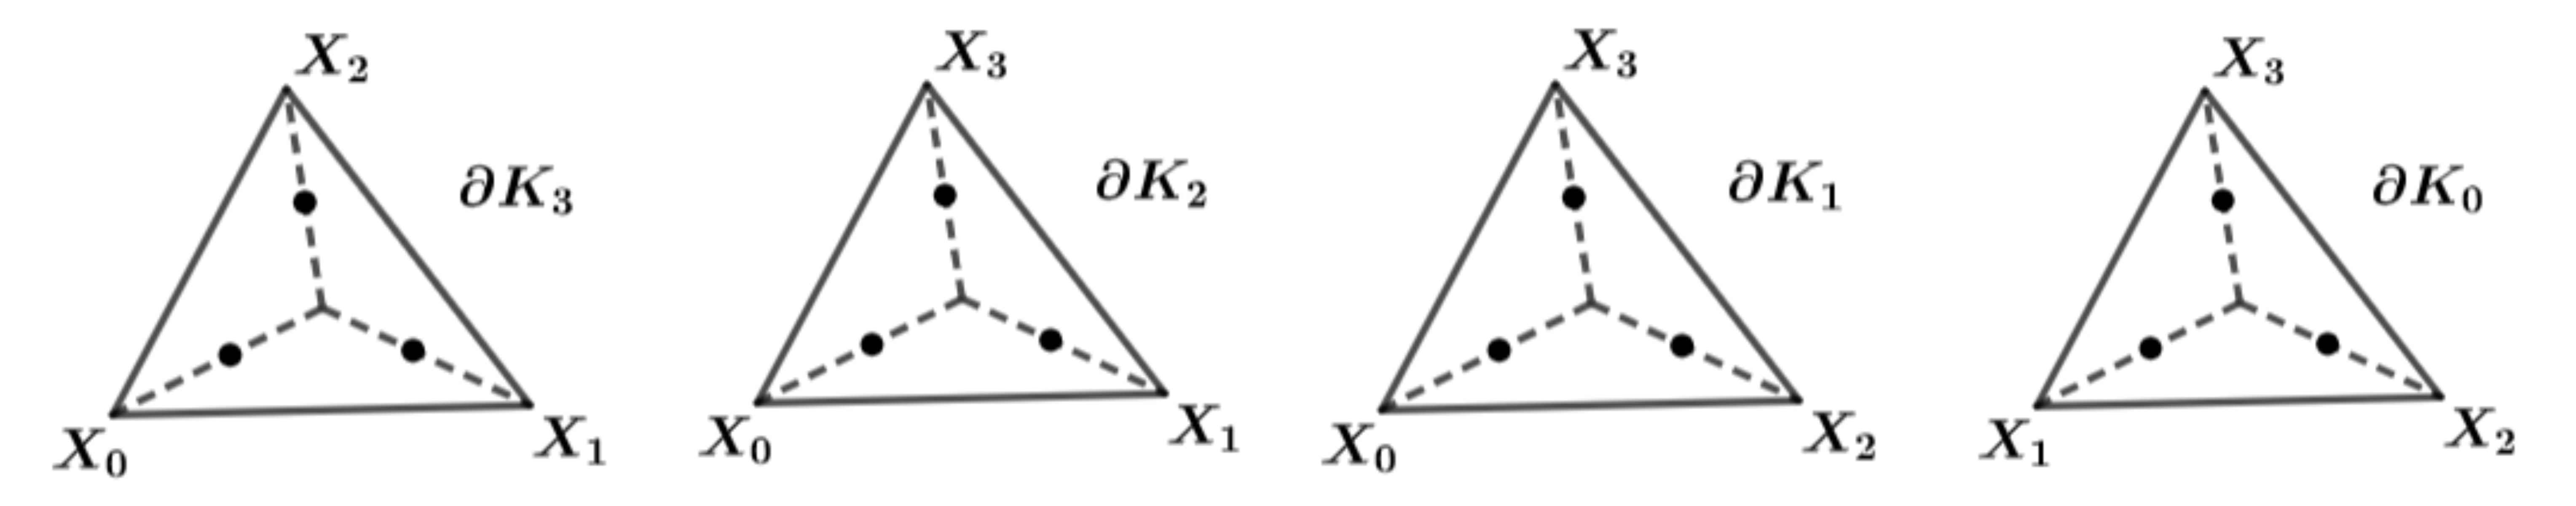
\includegraphics[width=0.9\textwidth]{images/2.jpg}
\caption{边界处的求积节点}
\label{IntegrationBoundaryPoint}
\end{figure}

定义单元边界点$\bs{X}$处的数值通量
\begin{equation}
\hat{\bs f}(\bs{X}, t)=\hat{\bs f}\left({\bs u_{h}^{K}\left(\bs{X}, t\right)}, {\bs u_{h}^{K'}\left(\bs{X}, t\right)}\right)
\end{equation}

其中$\bs u_{h}^{K}\left(\bs{X}, t\right)$ 与 $\bs u_{h}^{K'}\left(\bs{X}, t\right)$ 分别表示相邻单元$K$与$K'$上的数值解在$\bs{X}$处的取值,有
\begin{equation}
\bs{u}_{h}^{K}\left(\bar{\bs{X}}_{m}, t\right)=\sum\limits_{j=0}^{3} \bs{u}_{j}^{K}(t) \varphi_{j}^{K}\left(\bar{\bs{X}}_{m}\right)=\sum\limits_{j=0}^{3} \bs{u}_{j}^{K}(t) \hat{\varphi}_{j}\left(\bar{\bs{\eta}}_{m}\right)
\end{equation}

在计算$\bs{u}_{h}^{K'}\left(\bar{\bs{X}}_{m}, t\right)$时,需要用到点$\bar{\bs{X}}_{m}$在单元$K'$上对应的体积坐标。

实际计算中,常用 $LF$ 通量:
\begin{equation}
\hat{\bs f}(\bs{X}, t)=\frac{1}{2}\left[\bs f({\bs u_{h}^{K}\left(\bs{X}, t\right)}) \cdot \bs{n}+\bs f({\bs u_{h}^{K'}\left(\bs{X}, t\right)}) \cdot \bs{n}-{\alpha_{K}(\bs{X}, t)({\bs u_{h}^{K'}\left(\bs{X}, t\right)}-{\bs u_{h}^{K}\left(\bs{X}, t\right)})}\right]
\end{equation}
其中$\bs{n}=\left(n_{x}, n_{y}, n_{z}\right)$ 表示在四面体单元K的面上的单位外法向量
\begin{equation}\label{parameteralpha}
\alpha_{K}(\bs{X}, t)=\max \left\{\lambda\left({\bs u}_{h}^K(\bs{X}, t)\right), \lambda\left({\bs u}_h^{K'}(\bs{X}, t)\right)\right\}\\
\end{equation}
 $\lambda\left(\bs{u}\right)$为 $\displaystyle \frac{\partial (\bs{f}(\bs{u})\cdot \bs{n})}{\partial \bs{u}} $ 的谱半径,有
\begin{equation}\label{spectralradius}
{\lambda}(\bs{u})=|\bs{v} \cdot \bs{n}|+c_{s}=\Big|\frac{u_1}{u_0}n_x+\frac{u_2}{u_0}n_y+\frac{u_3}{u_0}n_z\Big|+c_s
\end{equation}
其中$\displaystyle c_{s}=\sqrt{\frac{\gamma{p}}{\rho}}$为声速。

\section{时间离散}
关于系数函数$\bs u_{j}^K(t), \forall K\in\mathcal T_h, j=0, 1, 2, 3$的常微分方程组\eqref{semidiscrete}可以将其简写为:
\begin{equation}\label{semidiscretescheme}
\frac{d \bs u_{j}^K(t)}{d t}=\bs L_{j}^K\big(\bs{u}_{h}^K(\bs{X}, t), \bs{u}_{h}^{K'}(\bs{X}, t), \bs{\beta}_{h}(\bs{X}, t)\big) \quad j=0,1,2,3 \quad \forall K\in\mathcal T_h
\end{equation}
其中,
\begin{equation}
\begin{split}
&\bs L_{j}^K\left(\bs u_{h}^{K}(\bs{X}, t), \bs u_{h}^{K'}(\bs{X}, t),\bs{\beta}_{h}(\bs{X}, t)\right)\\
= &\frac{|K|}{4a_j}\sum_{m=0}^{3}  \bs f\left(\bs u_{h}^K\left(\hat{\bs{X}}_{m}^K,  t\right)\right) \cdot \nabla \varphi_{j}^K\left(\hat{\bs{X}}_{m}^K\right)\\
- &\sum_{i=0}^{3}\frac{\left|\partial K_{i}\right| }{3a_j}\sum_{m=0}^{2} \hat{\bs f}\left(\bar{\bs{X}}_{m}^{\partial K_i}, t\right)\varphi_{j}^K\left(\bar{\bs{X}}_{m}^{\partial K_i}\right)
\end{split}
\end{equation}
$\bs{\beta}_{h}(\bs{X}, t)$ 表示数值解在计算区域的边界 $\partial \Omega$上的取值,由具体的边界条件给出,在紧邻边界的网格上计算数值通量时需要用到。

将要计算的时间区间$[0, T]$划分成剖分$0=t^0<t^1<\cdots<t^n<\cdots<t^N=T$, 记$\bs u_j^{K, n}$为系数函数$\bs u_j^K(t)$在任意$t^n$时刻的近似, 结合空间离散近似\eqref{spacediscritization}可得在$t^n$时刻解$\bs u(\bs{X}, t)$在单元$K$上的全离散近似为
\begin{equation}
\bs u(\bs{X}, t^n)\approx \sum\limits_{j=0}^3\bs u_j^{K, n}\varphi_j(\bs{X})
\end{equation}
为了求得所有的系数$\bs u_j^{K, n}$,我们采用二阶TVD Runge-kutta方法进行离散常微分方程组\eqref{semidiscretescheme},记第$n$步的时间步长$\Delta t^n=t^{n+1}-t^n$,那么$\bs u_j^{K, n}$的计算格式为
\begin{equation}
\begin{cases}
\displaystyle	   \bs u_{j}^{K,n+\frac{1}{2}}=\bs u_{j}^{K,n}+\Delta t^{n}\bs L_{j}^K\left(\bs u_{h}^{K, n}, \bs u_{h}^{K', n},\bs \beta_{h}\left(t^{n}\right)\right) \quad j=0,1,2 \\
\displaystyle	   \bs u_{j}^{K,n+1}=\frac{1}{2}\left(\bs u_{j}^{K, n}+\bs u_{j}^{K,n+\frac{1}{2}}\right)+\frac{1}{2} \Delta t^{n}\bs L_{j}^K\left(\bs u_{h}^{K, n+\frac{1}{2}}, \bs u_{h}^{K', n+\frac{1}{2}},\bs \beta_{h}\left(t^{n+1}\right)\right)
\end{cases}
\end{equation}
在上述推进计算中需给初始值 $\bs u_{j}^{K,0}$,根据初始条件$\bs{u}(\bs{X}, t=0)= \bs u_{0}(\bs{X})$,可设定初始值
\begin{equation}
\begin{aligned}
\bs{u}_{j}^{K, 0} & =\frac{1}{a_{j}} \int_{K} \bs{u}_{0}(\bs{X}) \varphi_{j}^{K}(\bs{X}) d \bs{X} \\
& \approx \frac{|K|}{4 a_{j}} \sum_{m=0}^{3} \bs{u}_{0}\left(\hat{\bs{X}}_{m}^{K}\right) \varphi_{j}^{K}\left(\hat{\bs{X}}_{m}^{K}\right) \\
& =\frac{|K|}{4 a_{j}} \sum_{m=0}^{3} \bs{u}_{0}\left(\bs{X}(\hat{\bs{\eta}}_{m})\right) \hat{\varphi}_{j}\left(\hat{\bs{\eta}}_{m}\right) \quad j=0,1,2,3
\end{aligned} 
\end{equation}
由于使用的是时间显格式,时间步长 $\Delta t^{n}=t^{n+1}-t^{n}$需满足限制条件
\begin{equation}
\displaystyle \Delta t^{n}=\frac{C F L}{\max\limits_{K \in \mathcal T_{h}}\Big[(\|\bs v\|+c_{s}) \cdot \frac{\text { surfacearea }(K)}{|K|}\Big]}
\end{equation}
其中,$ \displaystyle \frac{\text { surfacearea }(K)}{|K|}$ 为四面体单元K的表面积与体积之比,CFL条件数取0.3,
\begin{equation}
	\begin{split}
		\displaystyle c_{s}+\left\|\bs v\right\| \triangleq \sqrt{v_{1}^{2}\left(\bar{\bs u}_h^{K,n}\right)+v_{2}^{2}\left(\bar{\bs u}_h^{K,n}\right)+v_{3}^{2}\left(\bar{\bs u}_h^{K,n}\right)}+c_{s}\left(\bar{\bs u}_h^{K,n}\right) \quad \left(v_{1}, v_{2}, v_{3}\text { 表示速度 }\right)
	\end{split}
\end{equation}
其中,$\bar{\bs{u}}_{h}^{K, n}=\frac{1}{|K|} \int_{K} \bs{u}_{h}^{K, n}(\bs{X}) d \bs{X}=\bs{u}_{0}^{K, n}$ 为 $t^{n}$时的单元均值。

下面我们将每个单元$K$上的计算进行向量化。为此,我们记
\begin{equation}
\bs u^{K,n}=\begin{bmatrix}
\bs u_0^{K,n} & \bs u_1^{K,n} & \bs u_2^{K,n} & \bs u_3^{K,n}
\end{bmatrix}_{4\times 4},\quad \bs L^{K,n}=\begin{bmatrix}
\bs L_0^{K,n} &\bs L_1^{K,n} & \bs L_2^{K,n} & \bs L_3^{K,n}
\end{bmatrix}_{4\times 4}
\end{equation}
我们考虑$\bs L_{j}^K\left(\bs u_{h}^{K, n}, \bs u_{h}^{K', n},\bs \beta_{h}\left(t^{n}\right)\right)$的计算。我们有
\begin{equation}
\bs u_{h}^{K,n}\left(\bar{\bs{X}}_{m}^{\partial K_i}\right)=\sum\limits_{j=0}^3\bs u_j^{K,n}\varphi_j^K\big(\bar{\bs{X}}_{m}^{\partial K_i}\big)=\bs u^{K,n}\begin{bmatrix}
\varphi_0^K\big(\bar{\bs{X}}_{m}^{\partial K_i}\big)\\
\varphi_1^K\big(\bar{\bs{X}}_{m}^{\partial K_i}\big)\\
\varphi_2^K\big(\bar{\bs{X}}_{m}^{\partial K_i}\big)\\
\varphi_3^K\big(\bar{\bs{X}}_{m}^{\partial K_i}\big)
\end{bmatrix}=\bs u^{K,n}\begin{bmatrix}
\hat{\varphi}_0\big(\bar{\bs{\eta}}_{m}^{\partial K_i}\big)\\
\hat{\varphi}_1\big(\bar{\bs{\eta}}_{m}^{\partial K_i}\big)\\
\hat{\varphi}_2\big(\bar{\bs{\eta}}_{m}^{\partial K_i}\big)\\
\hat{\varphi}_3\big(\bar{\bs{\eta}}_{m}^{\partial K_i}\big)
\end{bmatrix}
\end{equation}
\begin{equation}
\begin{split}
\hat{\bs f}\left(\bar{\bs{X}}_{m}^{\partial K_i}, t^n\right)=&\frac{1}{2}\Big[\bs f\big({\bs u_{h}^{K,n}\left(\bar{\bs{X}}_{m}^{\partial K_i}\right)}\big)+\bs f\big({\bs u_{h}^{K',n}\left(\bar{\bs{X}}_{m}^{\partial K_i}\right)}\big) \Big]\cdot \bs{n}\\
-&\frac{\alpha_{K}(\bar{\bs{X}}_{m}^{\partial K_i}, t^n)}{2}\Big[{\bs u_{h}^{K',n}\left(\bar{\bs{X}}_{m}^{\partial K_i}\right)}-{\bs u_{h}^{K,n}\left(\bar{\bs{X}}_{m}^{\partial K_i}\right)}\Big]
\end{split}
\end{equation}
且根据定义\eqref{parameteralpha}以及谱半径表达式\eqref{spectralradius}可得
\begin{equation}
\begin{split}
\alpha_{K}(\bar{\bs{X}}_{m}^{\partial K_i},t^n)=\max \left\{\lambda\left(\bs u_{h}^{K,n}(\bar{\bs{X}}_{m}^{\partial K_i})\right), \lambda\left(\bs u_h^{K', n}(\bar{\bs{X}}_{m}^{\partial K_i})\right)\right\}
\end{split}
\end{equation}
\begin{equation}
\begin{split}
&{\lambda}(\bs u_{h}^{K,n}(\bar{\bs{X}}_{m}^{\partial K_i}))=\Big|\frac{u_1^{K,n}(\bar{\bs{X}}_{m}^{\partial K_i})}{ u_0^{K,n}(\bar{\bs{X}}_{m}^{\partial K_i})}n_x+\frac{ u_2^{K,n}(\bar{\bs{X}}_{m}^{\partial K_i})}{ u_0^{K,n}(\bar{\bs{X}}_{m}^{\partial K_i})}n_y+\frac{ u_3^{K,n}(\bar{\bs{X}}_{m}^{\partial K_i})}{ u_0^{K,n}(\bar{\bs{X}}_{m}^{\partial K_i})}n_z\Big|\\
&+\sqrt{\frac{\gamma (\gamma-1)\left(u_4^{K,n}(\bar{\bs{X}}_{m}^{\partial K_i})-\frac{1}{2{u_0^{K,n}(\bar{\bs{X}}_{m}^{\partial K_i})}} \left(( u_1^{K,n}(\bar{\bs{X}}_{m}^{\partial K_i}))^{2}+(u_{2}^{K,n}(\bar{\bs{X}}_{m}^{\partial K_i}))^{2}+(u_{3}^{K,n}(\bar{\bs{X}}_{m}^{\partial K_i}))^{2}\right)\right)}{u_0^{K,n}(\bar{\bs{X}}_{m}^{\partial K_i})}}
\end{split}
\end{equation}



\section{边界条件处理}
边界条件处理流体力学方程计算中边界条件通常有如下四种:
\begin{enumerate}
\item 周期边界:在我们的数值例子中,当计算边界上的数值流时,对应单元直接赋值即可;
\item 入流边界:密度、速度、压力这些物理量都已经指定好,直接使用这些物理量计算;
\item 出流边界:令边界外部的物理量值等于边界内部的值;
\item 反射边界,我们把边界内部的法向速度改变符号后赋给边界外部,而其他方向的速度、密度与压力复制给边界外部.

\end{enumerate}
在处理边界条件时有两种方法:
\begin{itemize}
	\item 将靠近$\partial\Omega$的单元K沿着边界处翻转过来,设置一个虚拟单元K',进行编号。跟区域$\Omega$内部的单元K一样,在K'上定义数值解。这样做的好处是:计算数值通量时,在区域$\Omega$的内部单元与边界单元处可以统一处理。
	
	\item 不设置虚拟单元,在区域边界$\partial\Omega$处计算数值通量时需用到数值解在边界外侧的极限值,它可以由边界条件直接给出。
\end{itemize}

\end{document}